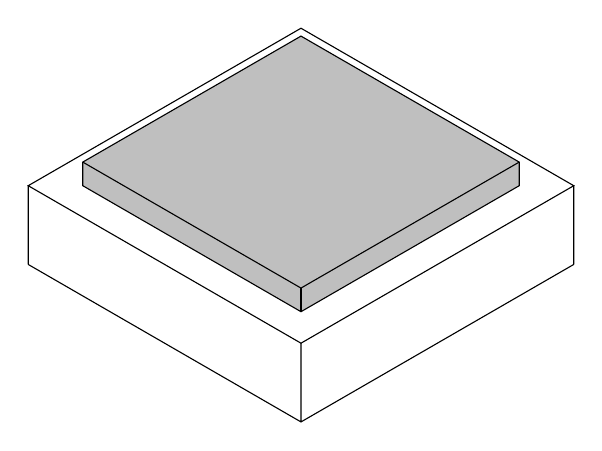
\begin{tikzpicture}
%top
\draw (0,0) ++ (0,-2) -- ++ (30:4) -- ++  (150:4) -- ++ (210:4) -- cycle;

%edges
\draw (0,-2) -- ++ (0,-1) coordinate (middle)
(0,-2) ++ (30:4) -- ++ (0,-1) coordinate (left)
(0,-2) ++ (150:4) -- ++ (0,-1) coordinate (right)
(left) -- (middle) -- (right);

%sample
\draw[fill = lightgray]
(0,-1.6) -- ++ (30:3.2) -- ++ (0,0.3) -- ++ (150:3.2) -- ++ (210:3.2) -- ++ (0,-0.3) -- cycle;
\draw
(0,-1.6) -- ++ (0,0.3);
\draw
(0,-1.3) -- ++ (30:3.2)
(0,-1.3) -- ++ (150:3.2);


\end{tikzpicture}